%!TEX root = ./seminar.tex
\section{The Future of Digital Healthcare}
\subsection{Secure Management of Patient Data}
With the digitization of healthcare environments a lot of patient data must be stored and accessed by algorithms. While this in itself is of less concern, security measurements need to be taken to prevent unauthorized access to this data. In addition, countries like Germany take confidentiality and security of data seriously and therefore have very strict regulations regarding storage, usage and even collection of this data \cite{dsgvo}. Regardless of security concerns, the race for your data has already begun, with Apple releasing Apple Health Record and Apple Watch with a single-lead ECG \cite{appleHealth}, joining Google with Google Fit and their WearOS - an operating system for smartwatches. Introducing Big Data concepts in the public healthcare sector may shift the focus from reactive to proactive care, reducing running costs and improving efficiency. This spans nearly all aspects of healthcare like diagnosis, treatment and population health management, to name a few. Furthermore, in moving from a volume-based to a value-based business model, healthcare providers see availability and accuracy of patients health data as pivotal. Now concerning security, healthcare data is stored in data centers with varying levels of security. They receive giant amounts of data from an even broader variety of sources. A first step to manage this data effectively and secure, is to introduce common data representations and local and regional standards. This allows the implementation of secure protocols for transportation and analysis in real-time. Currently, the healthcare industry is facing Distributed Denial of Service (DDoS) attacks, malware and social engineering attacks, among others. As Internet of Things environments are a big part of digital healthcare, their security is yet another problem, as implementing security in resource-constrained networks is an ever arising challenge. An approach would be to develop scaling key management solutions for secure transport of data in reasonable time-constraints. A last point, that is key to patient privacy and data confidentiality, is anonymization of data prior to analytics \cite{patil2014big}.
\subsection{Artificial Intelligence in Healthcare}
\label{sec:AIinHC}
Based on gathering and analyzing the vast amounts of data, powerful algorithms are now needed to ensure real-time and accurate usage to benefit patients in care. As the much praised (and feared) Artificial Intelligence (AI) expands its growth into the medical sector, patients already do, and further will, benefit from medical care that is tailored to their needs in a whole new way: proactively. Figure~\ref{fig:FDA_AI_Info} shows a timeline of Food and Drug Administration (FDA) approved AI-based algorithms in medicine since 2014 up until September 2019. Most of the algorithms are used in cardiology and radiology and are based on image procession.
This looks very promising, at least for the US healthcare environment. Meanwhile the current state in Germany is a bit less impressive. AI is used none the less, mostly for routine procedures and documentation, e.g. text assistance, error detection and detection of abnormalities to prevent fraud. More diagnosis-based tasks include scanning unobtrusive x-ray images for cancer detection, giving doctors more time to look into more urgent cases. But while better image processing software enters the market, a low degree of digitization prevents them from working effectively, again highlighting the importance of a solid foundation in data collection and management \cite{kiKroenung}. A promising application of AI is developed in stroke detection and treatment. Stroke is the leading cause of death in China and the fifth in North America. 85\% of strokes are caused by cerebral infarction. As early symptoms often are not detected properly, only few patients receive timely treatment. The possible solution consists of two Machine Learning (ML) algorithms, namely genetic fuzzy finite state machine and PCA, that are used in a movement-detecting device for early stroke prediction \cite{villar2015improving}. Meanwhile the diagnosis of stroke relies on neuroimaging techniques like MRI and CT. Here, studies used ML methods to assist stroke diagnosis, reaching an accuracy of almost 90\% \cite{rehme2014identifying}. \\
Predictions regarding the future of the use of AI in medical environments suggest that it will be mostly patient-driven, meaning that patients will use and benefit from AI-based medical services outside of hospitals and doctors offices as they become increasingly commercialized and open to the public. This would accelerate the degree of customized care, as these personal devices have maximal information about their user while communicating his or her troubles to the data centers of healthcare providers to get feedback, similar cases and possible treatment \cite{kiKroenung}.
\begin{figure}[htp]
    \centering
    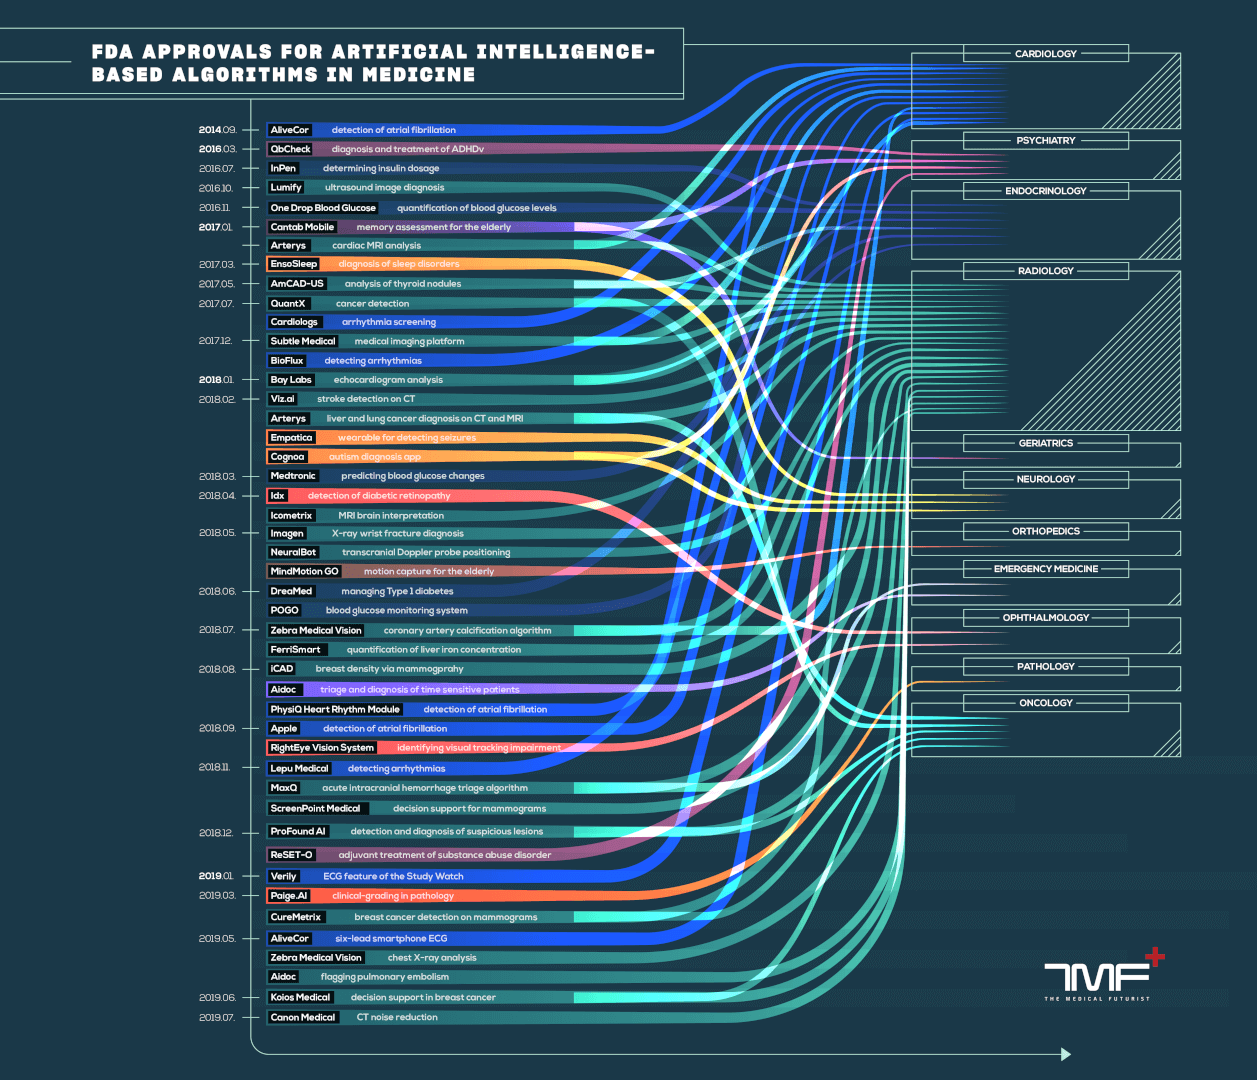
\includegraphics[width=\textwidth]{media/The-Medical-Futurist-FDA-approved-AI-algorithms-in-medicine-2019-09.png}
    \caption{FDA Approvals for Artificial Intelligence-Based Algorithms in Medicine - Infographic \cite{fdaAi}}%
    \label{fig:FDA_AI_Info}
\end{figure}
\subsection{Smart Implants}
While the previously mentioned wearable sensors can track a wide variety of health indicators, intrusive systems are on their way. Smart implants provide far more accurate stimuli and monitoring then vibration modules and sensors on the wrist can offer. Made from biocompatible material and equipped with low power microelectronics these devices can effectively transmit data from inside the body \cite{andreu2015wearable}. A prime example is an insulin implant that measures blood glucose levels in diabetics and releases insulin accordingly into the bloodstream \cite{rege2017development}. Another application is in surgery, monitoring white blood cells and neutrophil counts to prevent postoperative sepsis \cite{venema2013robustness}. Active and noninterruptible implants like pacemakers may be powered wireless by ultrasonic links doubling as a data communication path \cite{ozeri2010ultrasonic}.
\subsection{Value-Based Healthcare}
\label{sec:valueBasedHealthcare}
As populations worldwide get older, chronic diseases are more and more common. This includes cardiovascular diseases, Alzheimer's disease, diabetes and cancer. While these diseases are mostly incommutable, they are our leading killers and account for around 75\% of worldwide health expenditure \cite{tsiachristas2016financial}. People often do only die many years after diagnosis and while these diseases take a huge toll on their physical well-being, they also affect the mental health of the carriers themselves as well as that of their loved ones. So most of the time we live longer than 50 years ago, but this may not be a more fulfilling life, if half of it is spent with a chronic disease. A value-based approach to modern healthcare creates value "from health outcomes which matter to patients relative to the cost of achieving those outcomes [\dots] This concept [\dots] questions the need of aggressive, preventive or curative interventions which cost a lot but have few [positive] outcomes, while being ineffective and inefficient medical practice. On the other hand, this urges us to not seek for services to lower cost while sacrificing outcomes" \cite{putera2017redefining}. Of course this is far from the reality in healthcare environments at the moment, but any step into this direction is very likely to improve the life of patients as well as healthy individuals that are at risk of chronic diseases.
\subsection{Healthcare Through Education}
Health information provided by physicians, registered dietitians and other medical professionals is in general the best source, but in the more digitized world "Dr. Web" is becoming an ever increasingly consulted source. The ability for the masses of the 21th century to educate themselves about health is a phenomenal achievement. But sadly, as anyone who has tried to find a coherent answer or general consensus that is clearly laid out, may report: it is all a huge mess. While one can find details to every imaginable diet, exercise program and lifestyle online, the question what we should and should not do or eat is the battleground of a discussion that reaches across all aspects of health. Add some pseudo-science here, some unreliable sources there and you get a whole new lifestyle that a lot of people are willing to follow if you tell them they will be healthier eating steak all day \cite{carnivoreDiet}. Meanwhile, the WHO classifies red meat as a class 2A carcinogenic, saying that there is not enough evidence for causation, but a strong correlation was found \cite{whoRedMeat}. This results in a lot of confusion for consumers and poor health outcomes. Sadly, even heading to the local doctors office might not give a clear or qualified answer, as medical professionals in Europe receive on average just short of 24 hours of nutritional instruction during medical school \cite{chung2014nutrition}. The United States did even worse with just under 20 hours \cite{adams2010nutrition}. It seems like everyone has some work to do regarding nutrition, and this would very well pay of: adequate nutrition is one of the most powerful and easiest to incorporate things to fight, prevent and even reverse(!) chronic disease like coronary artery disease as Esselstyn et al. achieved to do. Following 32 months of a plant-based nutritional intervention without cholesterol-lowering medication, the severely impaired arteries (left) of their patients regained normal configuration (right) as can be seen in Figure~\ref{fig:reverseCAD}.
This demonstrates another case of Value-Based Healthcare~(cf. subsection \ref{sec:valueBasedHealthcare}) as nutritional advice is clearly a very cost efficient treatment in comparison to medication or surgery. Another takeaway is the problem that comes with the amount of available information in the digital age of the 21th century: spread of misinformation. A challenge for healthcare environments in the near future will be to establish clear recommendations and complete information about different approaches to "gain" health to alleviate consumers from confusion and providing evidence on which they can make more responsible lifestyle choices to improve their health outcomes. These recommendations may be derived from better designed clinical trials in form of randomized double blind placebo controlled studies, the consensus of good scientific work in intervention-based studies, to achieve meaningful results \cite{misra2012randomized}. Here hope lies in Artificial Intelligence~(cf. subsection \ref{sec:AIinHC}] which allows the detection of details that are missed by human-made analysis.
\begin{figure}[htpb]
    \centering
    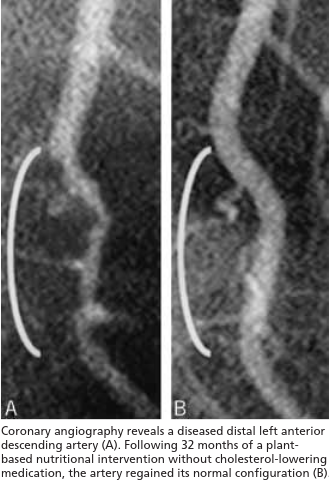
\includegraphics[width=0.8\linewidth]{media/Screenshot_2020-01-07_JFP_06307_Article1 pdf.png}
    \caption{A severely impaired artery on the left and the same artery 32 months later on the right \cite{esselstyn2014way}.}%
    \label{fig:reverseCAD}
\end{figure}
